\chapter{Desarrollo}
En este capítulo se detallara el proceso de desarrollo seguido dividido en \textit{sprints} como ya se ha comentado en la sección \nameref{sc:metodologia}.


\section{\textit{Sprint} 1}
Este primer \textit{sprint} tiene como objetivo general la investigación básica sobre la \acrshort{RI}. Sus objetivos concretos son: 

\begin{itemize}
	\item Leer el libro \acrlong{RI}: un enfoque práctico y multidisplinar \cite{RIspaBook}.
	\item Buscar los talleres \acrshort{BIR} centrándose en sus editoriales para realizar un listado priorizado por interés de los diversos artículos.
\end{itemize}

Siguiendo la recomendación de mi tutor (co-autor del libro) me centré en los capítulos \textit{"1 Introducción a la recuperación de información"}, \textit{"2 Indexación de documentos y procesado de consultas"}, \textit{"3 Modelos de recuperación de información clásicos"} y \textit{"10 Técnicas de modificación de la consulta"}. 

Esta lectura me hizo adquirir unas bases más teóricas a lo que ya había estudiado en la asignatura del máster \acrlong{GIW} donde obtuvimos una nociones básicas de lo que supone la \acrshort{RI} y sus vertientes realizando alguna práctica.

Los artículos de los talleres \acrlong{BIR} que encontré más destacados están detallados en el apartado \nameref{subsc:trabajosRelacionados}. Dichos trabajos se encuentran disponibles gratuitamente en \url{http://ceur-ws.org/} bajo el amparo de la Universidad Técnica de Aquisgrán (\textit{RWTH Aachen University}) en Alemania.

Cada una de las ediciones de estos talleres se encuentra estructurada dividida en diversos trabajos. Por un lado un editorial que resume la edición y todos los trabajos aceptados en la conferencia así como los trabajos individuales, alguna \textit{keynote} o presentación y algunas demostraciones. 

En este \textit{sprint} me dediqué a leer dichos editoriales clasificando por aparente interés los artículos de cada \acrshort{BIR} generando una lista priorizada utilizada como orden en el que estudiar los trabajos. En la siguiente imagen se puede apreciar el aspecto de dicha lista generada en \textit{Markdown}.

\begin{figure}[ht]
	
	\centering
	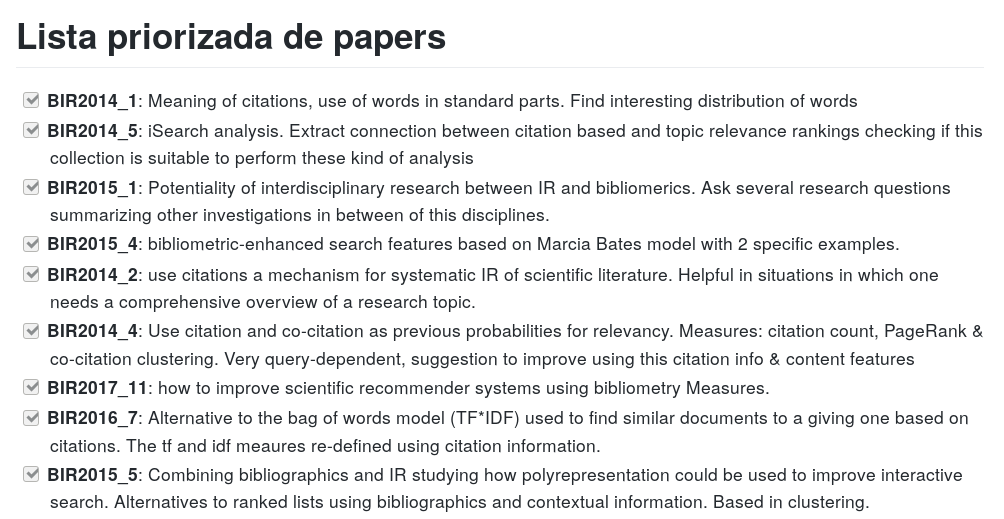
\includegraphics[width=\linewidth]{imagenes/lista_priorizada}
	\caption{Fragmento de la lista priorizada creada}
\end{figure}

\section{\textit{Sprint} 2}
Para el segundo \textit{sprint} plantee el indagar en la \acrshort{RI} e ir introduciendo la bibliometría. Sus objetivos concretos son: 

\begin{itemize}
	\item Leer los primeros papers de los \acrshort{BIR} resumiendo y extrayendo ideas interesantes para el proyecto.
	\item Buscar información sobre medidas bibliométricas (Citas, índice h combinado...)
\end{itemize}

A partir de la lista priorizada fui leyendo los primeros artículos, el orden de esta lista lo fui alterando ya que con frecuencia al indagar en el trabajo este perdía o incrementaba su interés. Con el objetivo de poder aprovechar más estas lecturas fui creando una especie de resúmenes en los que anotaba los puntos más importantes que se trataban en el artículo, otros artículos relacionados de los que se hablaba o los resultados obtenidos con su trabajo. En la siguiente imagen se puede apreciar uno de estos "resúmenes":

\begin{figure}[h!]
	
	\centering
	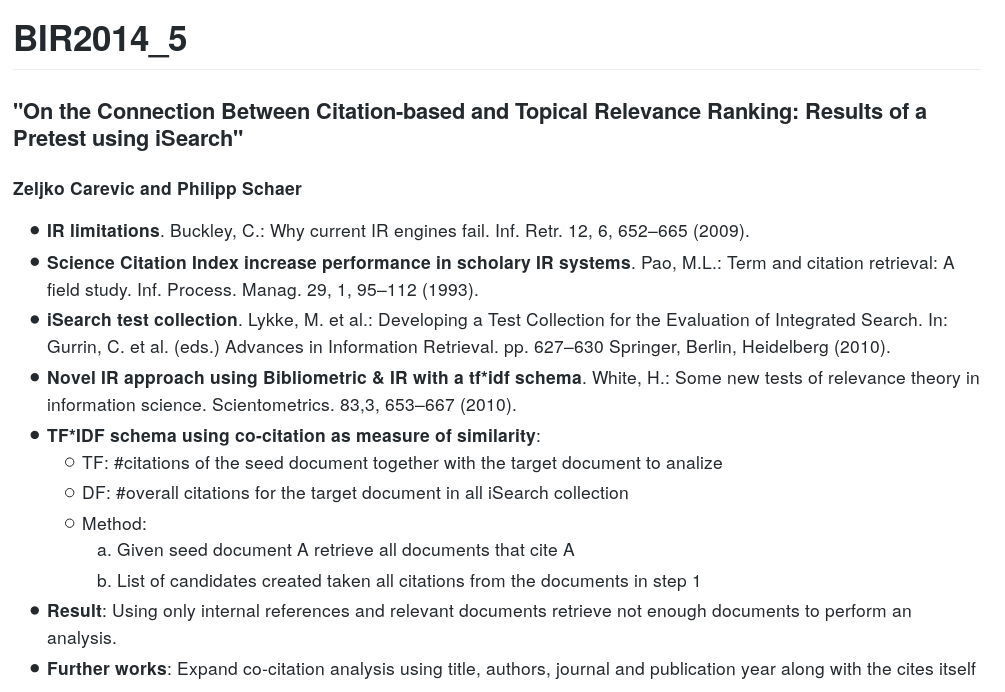
\includegraphics[width=\linewidth]{imagenes/paper_sumary}
	\caption{Ejemplo de resumen de uno de los papers}
\end{figure}

En este momento me empecé a introducir en el mundo de las medidas bibliométricas, ya que no tenía conocimiento previo alguno de que existiera esta disciplina siquiera, mediante la lectura de artículos iba descubriendo distintas medidas así como sus posibles aplicaciones a la \acrshort{RI} cuyo resultado final se encuentra sintetizado en la sección \nameref{sc:bibliometria}.

\section{\textit{Sprint} 3}
Ya en este punto decidí que estaba listo para ir documentando todo lo que había aprendido por ello en este \textit{sprint} me puse como objetivo escribir la introducción de este \acrshort{TFM}. Los objetivos concretos son:
\begin{itemize}
	\item Sintetizar mi estudio hasta este punto en los primeros capítulos de este \acrshort{TFM}.
	\item Pensar un enfoque para el proyecto a desarrollar decidiendo que clase de sistema se desarrollaría.
	\item Continuar leyendo algunos artículos más de los \acrshort{BIR}.
\end{itemize}

Para asimilar y reflexionar sobre todo lo que había leído me puse a escribir el capítulo Contexto e Introducción de este trabajo ya que ello me ayudaría a pensar un enfoque correcto. También quería poder mostrar algo a mi tutor para obtener algo de \textit{feedback} por su parte.

Continué leyendo algunos trabajos más con lo que dí por concluida mi proceso de investigación. Uno de esos últimos trabajos fue \cite{DBLP:conf/ecir/SarolLS18} el cual me gustó especialmente ya que pasaban de un modelo teórico a algo más práctico, accediendo a la \acrshort{API} de Scopus e incluyendo ejemplos de su implementación en un repositorio de \textit{GitHub} lo que me llevo a plantear mi modelo híbrido combinando el sistema habitual de un sistema \acrshort{RI} con reordenamiento de resultados \textit{a priori} usando medidas bibliométricas y un ordenamiento \textit{a posteriori} utilizando un grafo de citación entre los documentos.

Desgraciadamente estos enfoques dependen ampliamente de la cobertura de medidas bibliométricas disponibles, por ejemplo me hubiera encantado poder probar una reordenación previa utilizando alguna \textit{altmetric} como el número de lecturas o descargas de un artículo, pero la plataforma que he utilizado para extraer los artículos no dispone de dichas medidas.

\section{\textit{Sprint} 4}
\label{sc:sprint4}
Una vez sintetizado lo investigado y teniendo una idea aproximada de lo que pensaba desarrollar, en este \textit{sprint} me dispuse a realizar diversas pruebas que fueran definiendo las tecnologías a emplear, en concreto:
\begin{itemize}
	\item Buscar soluciones para montar sistemas \acrshort{RI}.
	\item Investigar como conectarse a la \acrshort{API} de Scopus o \acrshort{WoS}.
\end{itemize}

Estuve haciendo alguna pruebas con algunos \glspl{framework} de búsqueda. Ya había utilizado \textit{Lucene} como parte de las prácticas de la asignatura \acrshort{GIW}, pero me pareció demasiado bajo nivel así que me centré en investigar otras alternativas. Encontré que las principales, que casualmente utilizaban por debajo \textit{Lucene}, eran \textit{\textbf{Solr}} y \textit{\textbf{\acrfull{ES}}}.

Buscando alguna comparativa \cite{ES_Solr} y comentarios de usuarios en plataformas tan reputadas como \textit{StackOverflow} \cite{ES_Solr_SO} parecía que se recomendaba \acrshort{ES} por ser más sencillo de usar por lo que realicé un breve tutorial \cite{ES_tutorial} que me gustó bastante ya que resulta realmente simple de usar y basta únicamente con realizar consultas sobre una \acrshort{API} \acrshort{REST} por lo que basta con hacer peticiones \acrshort{HTTP} con algún cliente simple como \texttt{curl}. Todo esto hizo que me decidiera por este servidor de búsqueda.

Como ya comenté en el apartado \ref{ls:dataSourceAnalisis} realicé un análisis de diversas fuentes de datos y me decanté por seleccionar alguna que dispusiera de \acrshort{API}, en concreto Scopus ya que me resultó más rápido encontrar artículos que me servirían para mi colección documental. Por lo que comencé buscando la implementación que habían realizado en el artículo \cite{DBLP:conf/ecir/SarolLS18}, ya que en el mismo comentan que se encuentra disponible en \textit{GitHub} \cite{bir_scopus_gh}. Vi que dicha implementación era de muy bajo nivel, extraía los artículos mediante peticiones \acrshort{HTTP} y parseaban el \acrshort{XML} obtenido directamente. Pensé que tenía que haber un mejor método para esto, alguna librería que ya implementara los métodos de la \acrshort{API} y abstrayera de esas tareas. 

Así encontré la implementación oficial ofrecida por Elsevier, \texttt{elsapy} \cite{elsapy}, un modulo en \textit{python} que cuenta con diversas clases para modelar los tipos de documentos y permite obtener y parsear los datos de la \acrshort{API} de manera transparente. También encontré el módulo \texttt{scopus} \cite{scopus-api} una implementación alternativa que había comenzado a desarrollarse algo antes que la oficial, parecía más activa y contaba con mejor documentación incluyendo ejemplos bastante útiles. 

Funcionalmente \texttt{scopus} era muy similar a la versión oficial, pero estaba mejor modelada, se centraba solo en Scopus, que era lo que yo necesitaba, y tenia algunos añadidos muy útiles como uso de una caché por defecto con el objetivo de no repetir peticiones ya hechas, si no servirlas desde un documento almacenado en disco, lo que hacia increíblemente veloz la recuperación de entidades ya consultadas previamente así como gestión transparente de \acrshort{API} \textit{key}, basta con introducirla en la primera ejecución y la propia librería la guarda en un fichero interno el cual usa para su consulta el resto de ocasiones. Todo esto hizo que me decantara por esta última sobre la implementación oficial.

Para poder realizar mis pruebas tuve que solicitar una \acrshort{API} \textit{key} en el portal de Elsevier developers \url{https://dev.elsevier.com/myapikey.html} creando una cuenta gratuita. Para poder descargar los datos de Scopus desde fuera de la red de la universidad me ha sido necesario utilizar el servicio de \acrshort{VPN} de la \acrshort{UGR} siguiendo el siguiente tutorial \cite{vpnUGR}.

En la siguiente tabla se puede contemplar las distintas \acrshort{API}s de Scopus así como sus límites. En concreto he utilizado las \acrshort{API}s: \textit{Author Search} para realizar las búsquedas de autores, \textit{Author Retrieval} para obtener los datos completos de los autores y \textit{Abstract Retrieval} para obtener los artículos o \textit{abstracts}. 
Como se puede ver los límites de las \acrshort{API}s son bastante elevados 5000 peticiones semanales para la búsqueda y recuperación de autores así como 10000 para los \textit{abstracts}, por ello no han sido rebasados, pero en caso de sobrepasarlos bastaría con solicitar otra \acrshort{API} \textit{key} y cambiarla en el módulo \texttt{scopus}.

\begin{figure}[h]
	
	\centering
	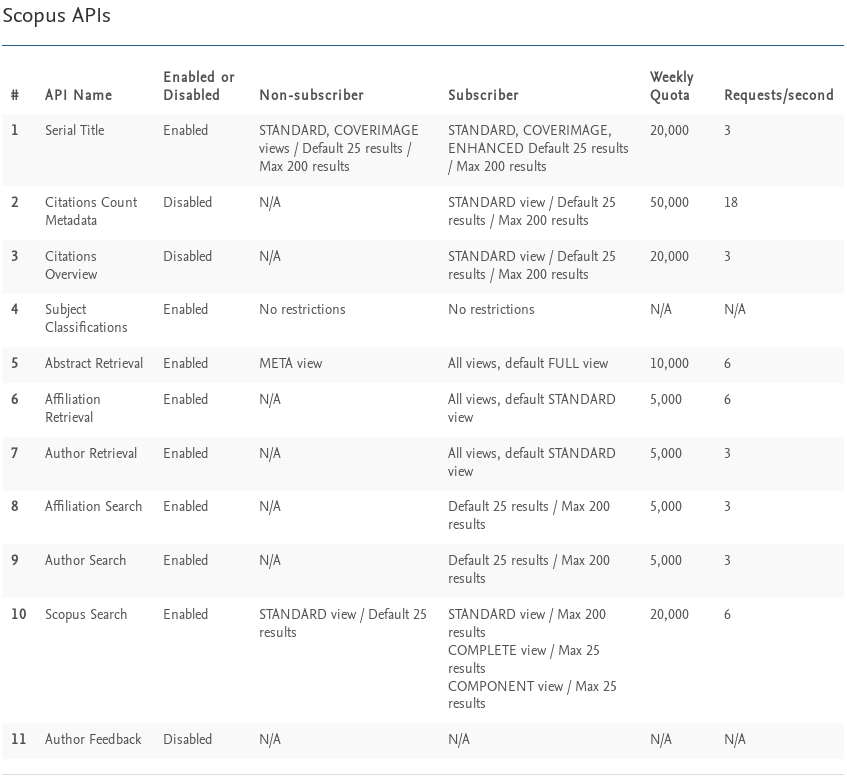
\includegraphics[width=\linewidth]{imagenes/scopusAPIs}
	\caption{ \acrshort{API}s de Scopus junto con sus límites}
\end{figure}
\section{\textit{Sprint} 5}
Tras toda la documentación e investigación previas en este punto realicé el proceso de obtención de datos. Dicho proceso fue dividido en 
\begin{itemize}
	\item Extraer información de los autores del ranking UGRinvestiga.
	\item Usar esos autores obtenidos para buscarlos en Scopus.
	\item Descargar todos los \textit{abstracts} de los autores obtenidos en el punto previo.
	\item Preprocesar y limpiar los datos obtenidos.
\end{itemize}

\subsection{Obtención de datos}

Teniendo en cuenta que no parecía haber opción de descarga de los datos del Ranking UGRinvestiga y que el formato parecía bastante estático con todos los datos en una tabla mi primer enfoque fue realizar un \gls{webscraping} utilizando la librería \texttt{BeautifulSoup} ya comentada previamente. El aspecto de la tabla se puede ver en la siguiente imagen.


\begin{figure}[h!]
	
	\centering
	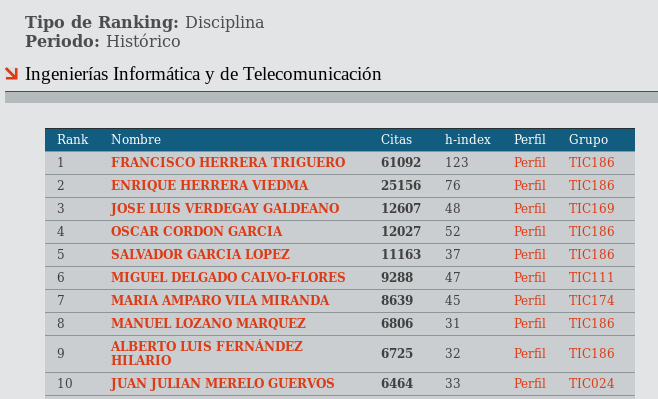
\includegraphics[width=0.9\linewidth]{imagenes/aspectoRankingUGRi}
	\caption{Aspecto tabla ranking UGRinvestiga}
\end{figure}

Realizando este proceso extraje datos de históricos y de los últimos 5 años de los autores de la facultad, además de aplicar este proceso al catálogo de grupos de investigación de Tecnologías de la Información y la Comunicación de la  \acrshort{UGR} para realizar un macheo por código de grupo con los datos del ranking.

Posteriormente dí con el proyecto OpenData de la \acrlong{UGR} el cual entre otros \textit{datasets} ofrecía el mencionado ranking actualizado a fecha 28 de Mayo de 2018 \cite{opendataUGR} en formato Excel, fácilmente legible y con algunos datos adicionales como el departamento de los autores, la url de Google Scholar de cada autor o su \textit{nick} el cual podía ser muy útil para buscarlos en Scopus.

Tras cargar estos últimos datos obtuve \textbf{214 autores} de la facultad. A continuación pasé al problema de buscar estos autores en Scopus, este problema no es nada trivial, ya que con frecuencia los autores no firman sus trabajos con su nombre completo, si no con parte de él o incluso de manera distinta entre unos trabajos y otros. Por ejemplo mi tutor, "JUAN MANUEL FERNÁNDEZ LUNA" suele firmar como Fernández Luna, Juan M. o como Fernández Luna, J.M.

El formato necesario para la búsqueda de autores en Scopus es nombre, apellidos y afiliación (la \acrshort{UGR} en este caso) por lo tanto primero me dispuse a extraer el nombre y apellidos a partir de la cadena completa que disponía, esto puede parecer sencillo, pero la riqueza del lenguaje español hace que existan apellidos compuestos o personas con segundos nombres lo que dificulta la tarea.

Estos problemas con los nombres me hicieron montar el siguiente algoritmo para intentar buscar un autor en Scopus:


\begin{algorithm}[h]
	\begin{algorithmic} 
		\ForAll {author in author\_list}
		\State $f\_name, l\_name \gets get\_name(author.nick)$
		\State $success, auth\_result  \gets author\_query(f\_name, l\_name)$
		\If {not success}
		\State $f\_name, l\_name \gets get\_name(author.full\_name)$
		\State $success, auth\_result  \gets author\_query(f\_name, l\_name)$
		\If {not success}
		\State $f\_name, l\_name \gets get\_name(author.name\_wo\_1\_lname)$
		\State $success, auth\_result  \gets author\_query(f\_name, l\_name)$
		\If {not success}
		\State $f\_name, l\_name \gets get\_name(author.name\_wo\_2\_lname)$
		\State $success, auth\_result  \gets author\_query(f\_name, l\_name)$
		\If {not success}
		\State $\textbf{return}\ No\ results\ found$
		\EndIf
		\EndIf
		\EndIf
		\EndIf
		\State $\textbf{return}\ auth\_result$
	
		\EndFor
	\end{algorithmic}  
	\caption{Obtiene los autores de Scopus a partir del ranking UGR}	
\end{algorithm}


Donde $f\_name$ y $l\_name$ hacen referencia a nombre y apellidos respectivamente y $name\_wo\_2\_lname$ hace referencia al nombre completo del autor eliminando el segundo apellido.

Con este algoritmo he logrado encontrar algún resultado en Scopus para \textbf{202 de los 214} autores buscados (\textbf{$\sim$ 94.39 \% de los autores}), a pesar de esto el número total de autores recuperados son 397, por lo que habrá que realizar una limpieza de los mismos.

\subsubsection{Limpieza de datos de autores}
Si observamos la distribución de \textbf{nacionalidades de los autores} recuperados, la cual se ve en la siguiente imagen se aprecia que hay una mayoría abrumadora de Españoles (como cabría esperar) pero también algunas nacionalidades inesperadas como Palestina o Australiana. Por ello consideraré que todo autor cuya nacionalidad no sea española debe haber sido recuperado incorrectamente y sera eliminado al tratarse de ruido, haciendo esto pasamos de 397 autores de Scopus representando a 202 autores de la \acrshort{UGR} a un total de 381 autores de Scopus respresentando a \textbf{198 autores de la \acrshort{UGR} ($\sim$ 98.02 \% de los 202 previos)}.

\begin{figure}[h!]
	
	\centering
	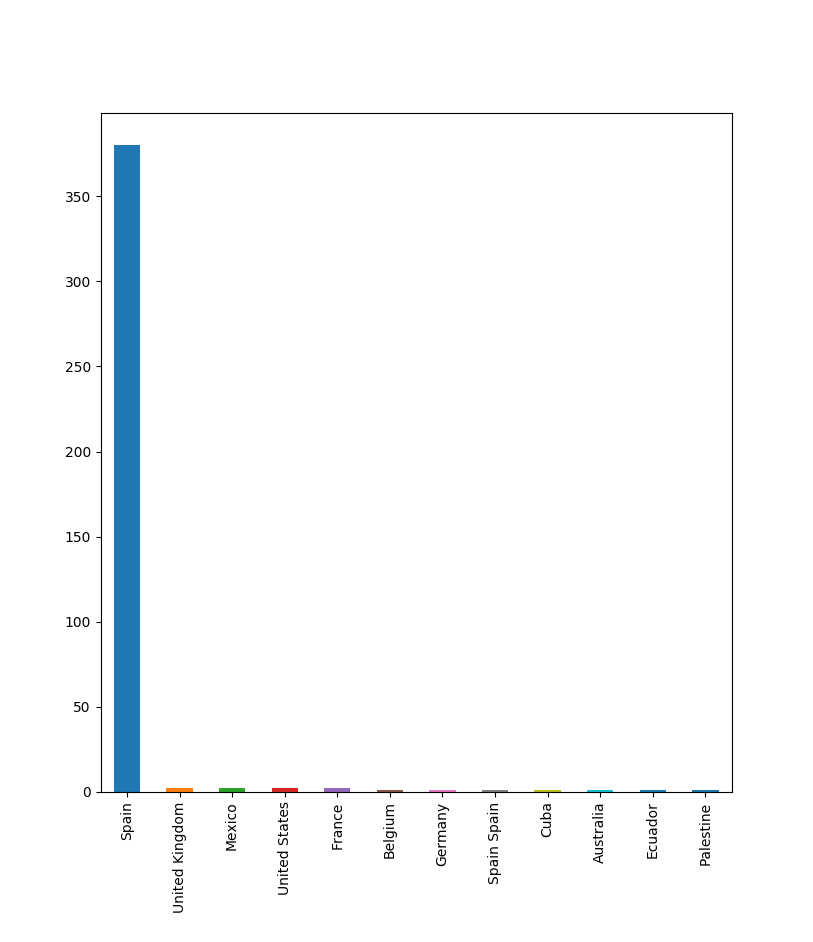
\includegraphics[width=0.9\linewidth]{imagenes/country_hist}
	\caption{Distribución de nacionalidades entre los autores recuperados}
\end{figure}

Continuando el filtrado si mostramos la distribución de \textbf{ciudades de los autores} restantes (ver la siguiente imagen) vemos que Granada o sus variantes aglutinan a la gran mayoría de los autores, por ello filtraré todos aquellos que no sean Granada lo cual me deja con un total de 334 autores de Scopus (\textbf{188 autores de la \acrshort{UGR} $\sim$ 94.95\% de los 198 previos}).

Por último he realizado un filtrado por \textbf{área del conocimiento} descartando aquellos autores que no tengan al menos un trabajo englobado en el área de Ciencias de la Computación (\textit{computer science}) con lo que finalmente me quedo con 199 autores de Scopus (\textbf{164 de la \acrshort{UGR}, $\sim$ 87.23 \% de los 188 previos})

\begin{figure}[h]
	
	\centering
	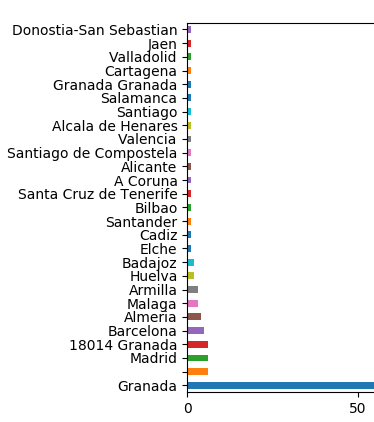
\includegraphics[width=0.5775\linewidth]{imagenes/city_hist}
	\caption{Fragmento de la distribución de ciudades entre los autores españoles recuperados}
\end{figure}
\newpage

En la siguiente gráfica represento un \textbf{\textit{clustering} de autores} \acrshort{UGR} donde aparecen etiquetadas las siguientes clases: la clase \textit{comp\_spa\_gr} representa a los autores que tienen algún autor en Scopus el cual es Español, de Granada y tiene algún artículo de Ciencias de la computación; la clase \textit{spa\_gr} igual con excepción del área del conocimiento, la clase \textit{spa} que tiene algún autor solo español y la clase \textit{other} que no cumple ningún criterio. Por tanto cada clase se ha ido eliminando en cada filtrado hasta quedarnos solo con la primera, la cual representa al \textbf{$\sim$ 81.19 \% de los autores totales de la \acrshort{UGR} (164 de 202 autores posibles)}.

\begin{figure}[h]
	
	\centering
	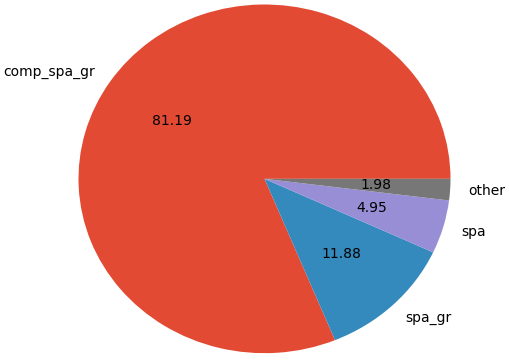
\includegraphics[width=0.5\linewidth]{imagenes/class_pie}
	\caption{Representación del clustering de autores llevado a cabo en la limpieza de datos}
\end{figure}

\subsubsection{Obtención de autores}
Esta limpieza se llevo acabo usando los resultados devueltos por la búsqueda de autores de Scopus (usando la clase \texttt{AuthorSearch} del paquete \texttt{scopus} la cual implementa la \acrshort{API} \textit{Author Search} de Scopus). Estos resultados de búsqueda contienen un subconjunto de los datos de autores disponibles, por lo que el siguiente paso fue descargar la ficha de cada uno de los 199 autores de Scopus usando para ello la clase \texttt{ScopusAuthor} del paquete \texttt{scopus} la cual implementa la \acrshort{API} \textit{Author Retrieval} de Scopus.

\subsubsection{Obtención de abstracts}
Una vez hecho esto me dispuse a llevar a cabo el grueso de la obtención de datos, la descarga de todos sus \textit{abstracts}. A partir de los autores de Scopus obtenidos previamente se obtienen todos los \texttt{eid} o \texttt{scopus\_id} de sus artículos con la clase \texttt{ScopusAuthor}. Utilizando esos identificadores recuperé todos los \textit{abstracts} usando la clase \texttt{ScopusAbstract} del paquete \texttt{scopus}, la cual implementa la \acrshort{API} \textit{Abstract Retrieval}, en su vista completa o \textit{full} \cite{scopusAbstractViews} ya que es la única que incluye las referencias, las palabras clave y las áreas del conocimiento de cada \textit{abstract}.

Los 199 autores recuperados cuentan con un total de 1263 artículos en Scopus, aunque este dato no es real, ya que frecuentemente los artículos tienen varios autores de entre esos 199, por lo que estos serían contados múltiples veces, el número de artículos únicos asciende a \textbf{891}.

\subsection{Preprocesado de los datos obtenidos}
En este punto había obtenido tres conjuntos de datos relacionados pero algo inconexos:
\begin{itemize}
	\item 164 autores del Ranking UGRinvestiga (tras la limpieza)
	\item 199 autores de Scopus (tras la limpieza)
	\item 891 \textit{abstracts} de Scopus. 
\end{itemize}

El primer paso como parece lógico fue combinar los autores de la \acrshort{UGR} y Scopus, el numero de estos no coincide ya Scopus a veces no es capaz que dos autores son la misma persona si firma de distinta manera, por ello crea dos autores distintos.

Para realizar esta combinación agrupé los autores de Scopus por el ID \acrshort{UGR} sumando el número de documentos y de citas de los autores individuales seleccionando el mayor índice h individual entre ellos. A continuación mezclé estos 164 autores combinados de Scopus con los datos provenientes del Ranking UGRinvestiga y del nombre del grupo de investigación, quedando finalmente constituida la entidad de datos descrita en la sección \nameref{subsc:author} del capítulo Diseño. Dicha entidad se encuentra implementada en la clase del modelo \texttt{Author} y ha sido introducida en la \acrshort{BD} \textit{MongoDB} en la colección \textit{author}.

En los \textit{abstract} emulé el proceso de combinación de autores asignando los artículos al mismo autor \acrshort{UGR} aunque originalmente fueran de distintos autores Scopus. 

Tras ello limpié las referencias de cada uno de ellos para mantener solo las referencias a artículos que formaban parte de la colección, eliminando las referencias a otros trabajos externos. Esto puede suponer una perdida de información, ya que limitaría el análisis de co-citación, pero hace más manejable el conjunto de referencias y como se comprueba en \cite{DBLP:conf/ecir/SarolLS18} cuando más directa sea la relación de citación, más útil resulta para este análisis. Aplicando esta limpieza se mantienen un total de \textbf{742} referencias, quedando con esto la entidad descrita en la sección \nameref{subsc:abstract} del capítulo Diseño. Dicha entidad se encuentra implementada en la clase del modelo \texttt{Abstract} y ha sido introducida en la \acrshort{BD} \textit{MongoDB} en la colección \textit{abstract}.



Como curiosidad de este \textit{sprint} me gustaría destacar que durante mi investigación de los datos devueltos por Scopus sobre los \textit{abstracts} me percaté que la librería \texttt{scopus} no parseaba las palabras clave de los mismos aunque estas aparecían en los \acrshort{XML} obtenidos de la \acrshort{API}, estas palabras clave podían funcionar bien en los sistema de búsqueda, como había leído durante mi proceso de documentación, por ello añadí esa funcionalidad a la librería y dicho cambio fue \href{https://github.com/scopus-api/scopus/pull/68}{incorporado a la misma} en su versión 0.9.

\section{\textit{Sprint} 6}
Una vez tenía los datos preparados en este sprint me marqué como objetivo crear un sistema de búsqueda básico por contenido (sin aplicar bibliometría). Este objetivo se descompuso en:
\begin{itemize}
	\item Indexar los datos en \acrlong{ES}.
	\item Crear un cliente web que permita la búsqueda usando \acrshort{ES}.
	\item Crear un servidor \gls{backend} como apoyo al proceso de búsqueda que permita recuperar los datos completos, no solo los indexados.
\end{itemize}

\subsection{Indexación de los datos}
Tras analizar un par de alternativas como motores de búsqueda (ver \nameref{sc:sprint4}) me decanté por utilizar \acrshort{ES}. Tras realizar un breve tutorial me pareció muy manual el proceso de introducir datos por lo que busqué alguna forma de hacerlo programáticamente. En mi búsqueda dí con el tutorial \cite{indexingES}, que utilizaba el cliente oficial de \acrshort{ES} en \textit{python} \texttt{elasticsearch-py} \cite{ES_client}. Usando dicho tutorial como base y realizando un mapeo del índice \footnote{Forzar los datos y tipos de estos en un índice, lo cual no es necesario ya que \acrshort{ES} es capaz de gestionarlo dinámicamente, pero con ello se consigue aplicar estrategias de búsquedas específicas para los tipos de datos y hace que no se pueda introducir un documento distinto por error}\cite{mappingES} creé los índices \textit{author} y \textit{abstract}.

No todos los datos de dichas entidades han sido indexadas, ya que hay algunas que no aportaría nada a la búsqueda, es más solo la entorpecería al ocupar un espacio innecesario en el índice. Por ejemplo los identificadores o \acrshort{URL}s no aportan nada.

El índice \textit{author} está constituido por los campos útiles para la búsqueda de contenido (de tipo \textit{text}) y los campos de medidas bibliométricas para poder ordenar o aplicarlos en la búsqueda bibliométrica. En la siguiente tabla se recoge los campos concretos de la clase \texttt{Author} que forman parte del índice homónimo:

\begin{table} [h!]
	\centering
	\begin{tabular}{| c | c |}
		\hline
		\textbf{Campo}                & \textbf{Tipo}    \\ \hline
		\textit{full\_name}           & \textit{text}    \\
		\textit{nick\_name}           & \textit{text}    \\
		\textit{scopus\_cites}        & \textit{integer} \\
		\textit{scopus\_hindex}       & \textit{integer} \\
		\textit{speciality}           & \textit{text}    \\
		\textit{num\_docs}            & \textit{integer} \\
		\textit{investigation\_group} & \textit{text}    \\
		\textit{ugr\_hindex}          & \textit{integer} \\
		\textit{ugr\_cites}           & \textit{integer} \\
		\textit{ugr\_hindex5}         & \textit{integer} \\
		\textit{ugr\_cites5}          & \textit{integer} \\ \hline
	\end{tabular}
	\caption{Campos del índice \textit{author}}
\end{table}

\newpage
Respecto al índice \textit{abstract} los campos específicos son:

\begin{table} [h!]
	\centering
	\begin{tabular}{| c | c |}
		\hline
		\textbf{Campo}             & \textbf{Tipo}    \\ \hline
		\textit{title}             & \textit{text}    \\
		\textit{abstract}          & \textit{text}    \\
		\textit{authors}           & \textit{text}    \\
		\textit{subject\_areas}    & \textit{text}    \\
		\textit{keywords}          & \textit{text}    \\
		\textit{publisher}         & \textit{text}    \\
		\textit{publication\_name} & \textit{text}    \\
		\textit{cites}             & \textit{integer} \\
		\textit{date}              & \textit{date}    \\ \hline
	\end{tabular}
	\caption{Campos del índice \textit{abstract}}
\end{table}


\subsection{Desarrollo del buscador por contenido}
Teniendo en cuenta la características del proyecto cuyo objetivo es desarrollar un prototipo, el diseño no era un punto primordial, pero también quería crear un cliente que fuera fácilmente usable. Esto hizo que me decantara por crear un cliente web, ya que trabajo como desarrollador \textit{full-stack} y es un ambiente en el que me muevo cómodo y me permitiría desarrollar algo sin la necesidad de aprender tecnologías muy distintas.

Por eso comencé buscando librerías que facilitaran el desarrollo de interfaces de usuario para sistemas basados en \acrshort{ES}. Me topé con dos destacadas \textit{Searchkit} \cite{searchKit} y \textit{Reactivesearch} \cite{reactiveSearch}, ambas basadas en el \gls{framework} \textit{ReactJS}. Básicamente suponen un conjunto de componentes visuales ya construidos (filtros, barras de búsqueda...), \textit{layouts} y otras utilidades adicionales que facilitan la comunicación con \acrshort{ES}.

Ojeando las documentaciones y ejemplos me dió la impresión de que \textit{Reactivesearch} parecía más completa y customizable, con más componentes y opciones de diseño, pero es desarrollada por appbase.io, una plataforma de \acrshort{DBaaS} y la documentación de \textit{Reactivesearch} se orienta mucho a que desarrolles aplicaciones de búsqueda utilizando su plataforma como fuente de datos, lo cual me echó algo para atrás. Por otro lado \textit{Searchkit} parecía más simple, con menos componentes y opciones pero funcionales, ideal para mí ya que no buscaba realizar una interfaz gráfica compleja, si no simple, contaba con ejemplos en vivo y proyectos de ejemplo demostrando la funcionalidad de cada uno de sus componentes.

Por todo ello decidí utilizar \textit{Searchkit}. En la siguiente imagen se puede apreciar el aspecto de la demo de esta librería, como se puede observar cuenta con una interfaz bastante simple, muy inspirada en \textit{Material Design} \cite{materialDesign} y con unas zonas claramente diferenciadas: En rojo podemos ver una barra superior con el nombre de la aplicación y la barra de búsqueda, a la izquierda en amarillo una zona de filtros, en recuadros azules un par de barras que muestran información sobre los resultados de búsqueda y permiten modificar la ordenación o visualización; por último en verde aparece la zona de resultados.

\begin{figure}[h]
	
	\centering
	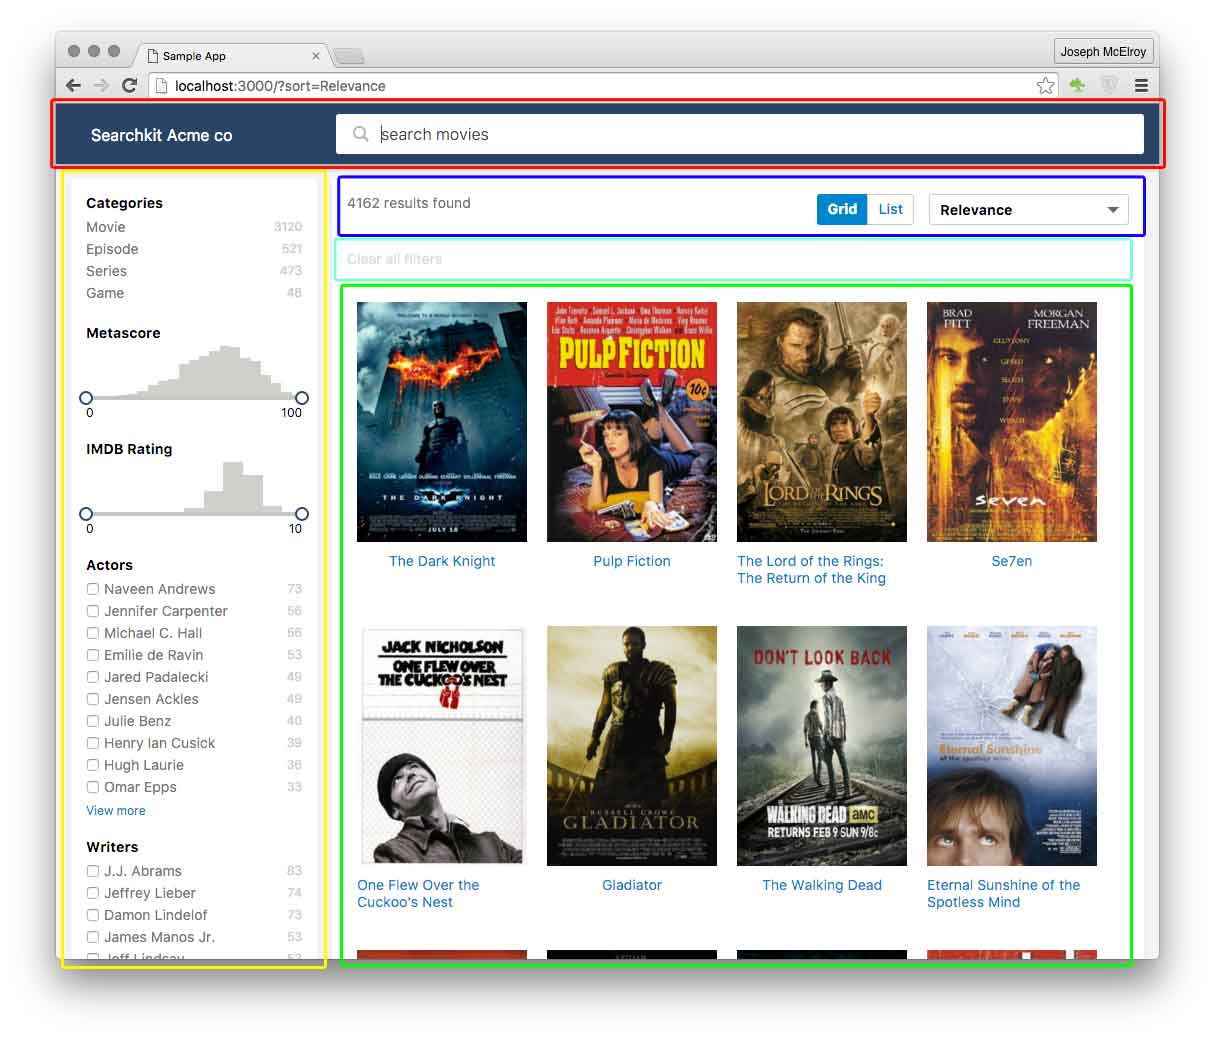
\includegraphics[width=\linewidth]{imagenes/AspectDemoSearchKit}
	\caption{Aspecto demo \textit{Searchkit}}
\end{figure}

Para mi aplicación seguiré este esquema a excepción de la zona de filtros amarilla ya que el pretendo que el la búsqueda sea lo más simple posible.

Habilitar la conexión entre \acrshort{ES} y \textit{Searchkit} es realmente sencillo, basta con instanciar un objeto \texttt{SearchkitManager} y pasarlo como argumento al componente \textit{React} \texttt{SearchkitProvider} que englobe todos los componentes de \textit{Searchkit} como si se tratara de un contexto. En el siguiente bloque de código se puede contemplar como se realiza la conexión con el índice de \textit{author} de \acrshort{ES}.

\newpage

\begin{lstlisting}[style=htmlcssjs, caption=Conexión de \textit{Searchkit} a una instancia \acrshort{ES} local]
const searchkit = new SearchkitManager("http://localhost:9200/author")


<SearchkitProvider searchkit={searchkit}>
...
</SearchkitProvider>
\end{lstlisting}

Además de esto al conectarnos con una instancia local es necesario activar las opciones de \acrshort{ES} relacionadas con CORS como la documentación oficial aclara \cite{searchKit_cors}.

Además de \textit{Searchkit} también he utilizado el \gls{framework} \textit{MaterialUI} para algunos de los componentes visuales como las \textit{tabs} de selección de búsqueda de autores o \textit{abstracts} o los botones que aparecen en la aplicación.

Esta imagen muestra el aspecto que tiene el buscador de autores, como se puede ver la interfaz es realmente sencilla contando unicamente con una barra de búsqueda, unas pestañas para cambiar entre búsqueda de autores o artículos y las propias vistas de resultados así como un selector de orden de los mismos.


\begin{figure}[h]
	
	\centering
	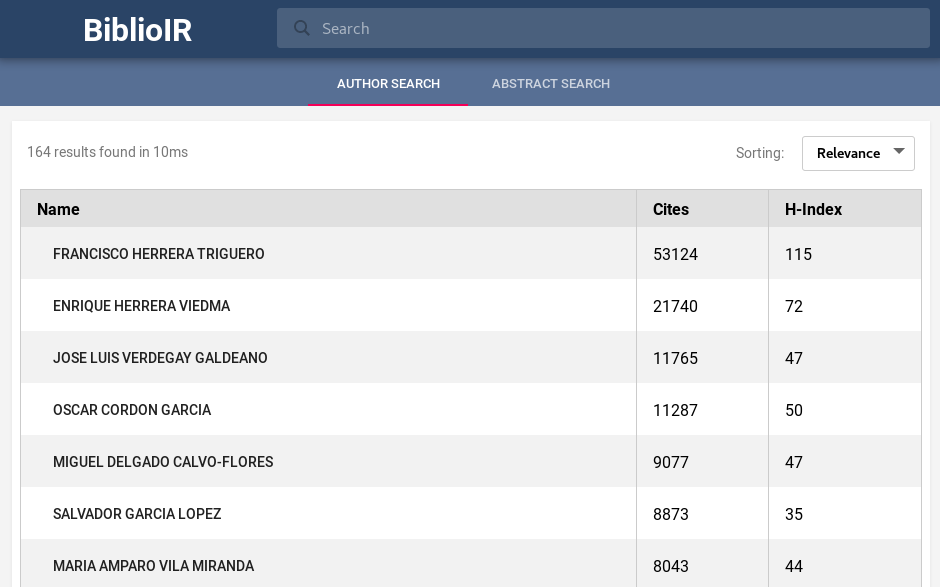
\includegraphics[width=\linewidth]{imagenes/AspectoBuscadorAutores}
	\caption{Aspecto buscador de autores}
\end{figure}
\newpage
Al seleccionar cualquiera de los autores haciendo click en su nombre podemos ver una ficha detallada con todos los datos de la clase \texttt{Author} incluyendo botones a los perfiles disponibles del autor.

\begin{figure}[h]
	
	\centering
	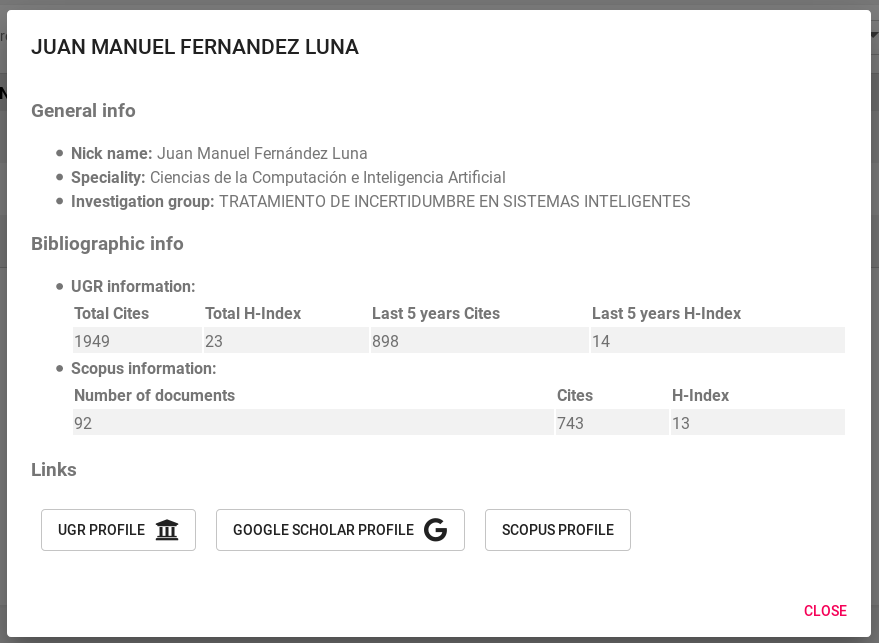
\includegraphics[width=\linewidth]{imagenes/AspectoVistaAutor}
	\caption{Aspecto vista de un autor}
\end{figure}

\newpage

Por otro lado la vista del buscador de \textit{abstracts} es algo diferente ya que no muestra los resultados en una tabla, si no a modo de lista. Para cada uno de los artículos se puede observar unos datos básicos: su título, autores, fecha de publicación, citas y palabras clave.

\begin{figure}[h]
	
	\centering
	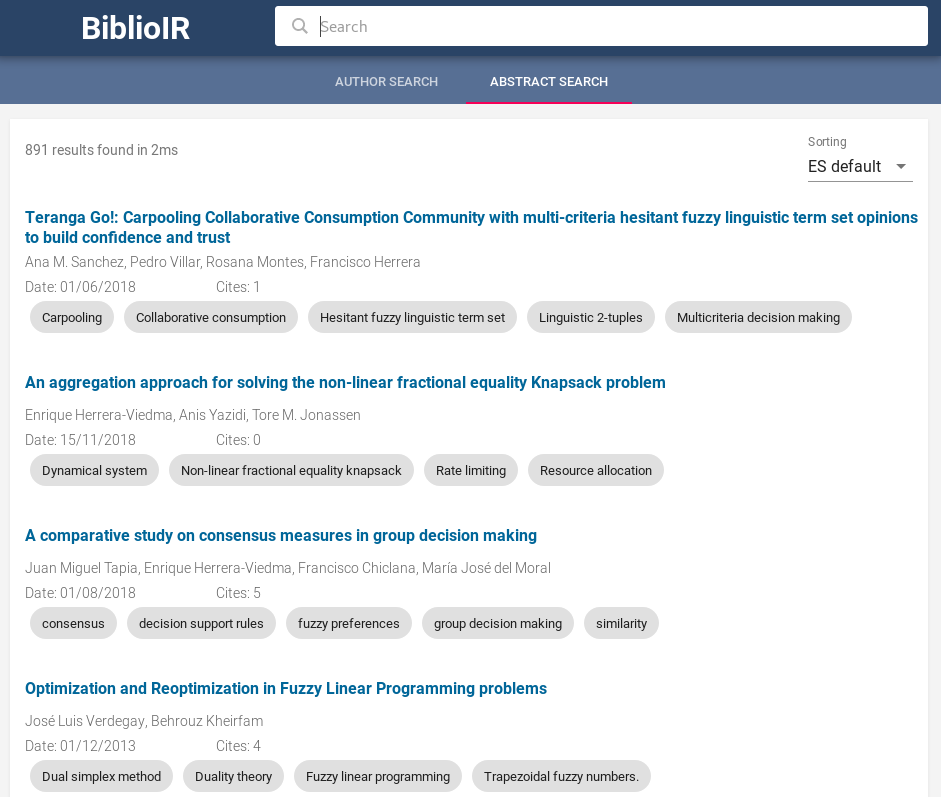
\includegraphics[width=\linewidth]{imagenes/AspectoBuscadorAbstracts}
	\caption{Aspecto buscador de artículos}
\end{figure}

\newpage

Como cabe esperar también se dispone de una vista detallada de cada artículo, donde se muestran datos más detallados, el\textit{abstract} o en enlace del mismo en Scopus.
\begin{figure}[h]
	
	\centering
	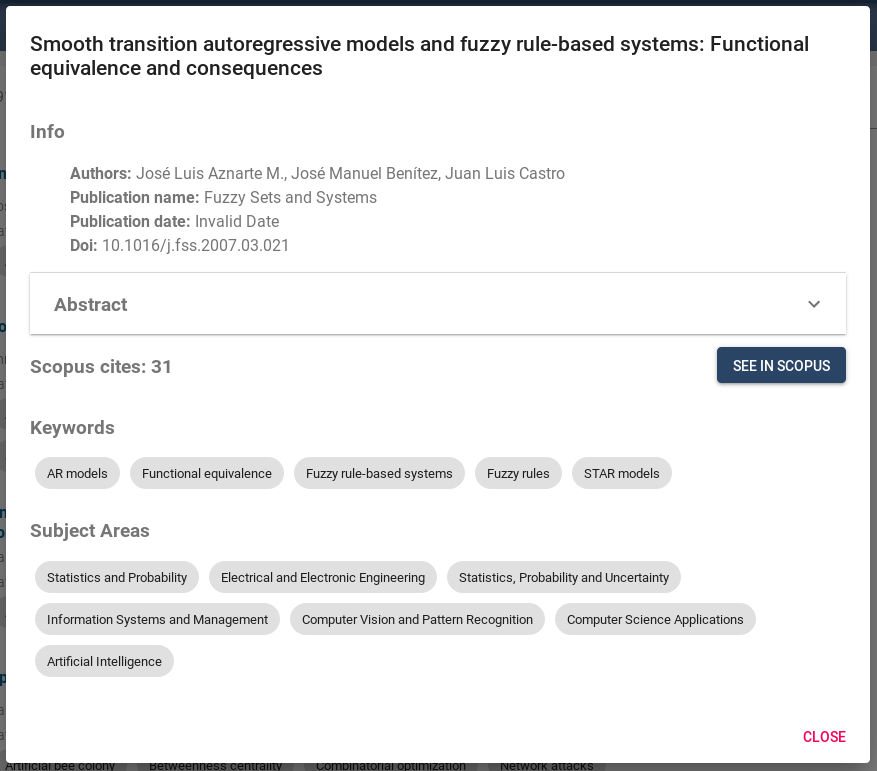
\includegraphics[width=\linewidth]{imagenes/AspectoVistaAbstract}
	\caption{Aspecto vista de un artículo}
\end{figure}

Además de todo este \gls{frontend} he desarrollado un pequeño servidor utilizando \textit{Flask} que permite recuperar los datos completos de un autor o artículo por su id para combinarlos con los que vienen de \acrshort{ES} y poder desplegar las vistas detalladas de cada elemento que se han mostrado antes. También cuenta con servicio para obtener un diccionario de artículos por id de Scopus y así poder mostrar una sección de referencias en los artículos que las tengan con enlaces directos a sus referencias.

\section{\textit{Sprint} 7}
Con toda la infraestructura de búsqueda ya funcionando había llegado la hora de aplicar medidas bibliométricas para mejorar la búsqueda así como documentar lo hecho hasta ahora. Este objetivo se se divide por tanto en:
\begin{itemize}
	\item Investigar como modificar la puntuación asignada por \acrshort{ES} a los documentos.
	\item Combinar esa puntuación con medidas sobre las citas e índices h.
	\item Documentar lo desarrollado hasta ahora.
\end{itemize}

\subsection{Aplicación de medidas bibliométricas y ordenación de resultados}
\acrlong{ES} provee una puntuación o \texttt{\_score} en cada documento devuelto por cada consulta. Dicha puntuación está basada en el propio modelo de \textit{Lucene}, el cual se explica brevemente en la documentación oficial de \acrshort{ES} \cite{ES_scoring}. Básicamente supone la combinación de varios modelos clásicos explicados en el apartado \nameref{subsc:modelos}. 

Primero se ejecuta un modelo booleano para descartar documentos que pueden formar parte del resultado de la consulta, tras esto para ordenar por relevancia este subconjunto de documentos se utiliza el modelo vectorial con un esquema de pesos \textit{tf*idf} modificado con una normalización en función de la longitud del campo (a campo más corto, más relevancia) además de algunas otras modificaciones, como los campos que el usuario haya decidido priorizar.

Todo esto hace que esta puntuación sea muy dependiente de la consulta y no tenga un límite superior, ya que eso significaría que se puede determinar la relevancia absoluta dada una consulta, cosa que no es posible como ya he discutido en los comienzos de esta memoria. 

Por suerte en \acrshort{ES} esta contemplada la posibilidad de modificar esta puntuación de manera interna usando lo que se conoce como \textit{Function Score Query} \cite{ES_func_score}, simplemente en la propia consulta se determina como se quiere modificar dicha puntuación. Dispone de bastante flexibilidad, permite reemplazarla por completo, combinarla mediante una suma, media o multiplicación con otras medidas como por ejemplo una función sobre un campo del documento (como puede ser las citas) o cualquier función calculable con un \textit{script}. 

Esta fue mi primera opción con la que estuve probando logrando realizar combinaciones. Logre probar algunos ejemplos prometedores pero no tenía claro como combinar ya que por ejemplo la puntuaciones que \acrshort{ES} asignaba en mis pruebas a los documentos solían ser pequeñas (menores que 10) y aplicarle alguna modificación con el campo de las citas (que llega a superar las centenas) hacía que prácticamente diera igual la consulta, los resultados siempre eran un listado ordenado por citas ya que su peso era mucho mayor que todo el mecanismo de puntuación interno de \acrshort{ES}. Por ello me puse a buscar como normalizar las puntuaciones internas entre 0 y 1 para aplicar yo también una normalización a las citas y poder combinar ambas medidas con igual peso cada una. Tras navegar por varia preguntas en \textit{StackOverflow} que aplicaban diversos trucos que no llegaban a funcionar dí con una \textit{feature request} en el propio repositorio \textit{GitHub} de \acrshort{ES} \cite{ES_normalize_score} donde los autores afirmaban que no se trataba de una buena idea y simplemente se limitaban a cerrar.

Esto hizo que me planteara un enfoque más manual, si no podía combinar a mi gusto las puntuaciones en \acrshort{ES} podría obtener las puntuaciones de los documentos en el \gls{frontend}, normalizar por la máxima puntuación para la consulta y tras esto combinar con mis medidas. 

Para llevar a cabo este enfoque lo primero que realicé fue normalizar los números de citas e índices h para introducirlos como nuevos campos precalculados en los índices ya creados, por ello creé los campos \texttt{cites\_norm} y \texttt{hindex\_norm} en el índice de autores y los homólogos en el de artículos, con la excepción de que el índice h de un artículo no es algo real, ya que esta medida se aplica a los autores, pero para poder aplicarlo realice una normalización de la media de los índices h de los autores del artículo.

Teniendo ya ambas medidas normalizas tenia que establecer el método de combinación, siguiendo el consejo de mi tutor implementé dos combinaciones que han sido ampliamente utilizadas y estudiadas para este tipo de problemas, los algoritmos \texttt{CombMAX} y \texttt{CombSUM} \cite{DBLP:conf/trec/ShawF94}. El primero es básicamente seleccionar el valor máximo en N rankings de puntuación normalizados para cada uno de los documentos mientras que el segundo supone la suma de las N puntuaciones normalizadas para cada documento. 

Estas son todas las piezas para la aplicación de medidas bibliométricas en mi sistema, el mecanismo por tanto es el siguiente:

Cada consulta $q$ devuelve un conjunto de documentos ordenados por el mecanismo interno de \acrshort{ES} $\{d_1, d_2, ..., d_n\}$ cada uno de los cuales cuenta con una puntuación $s$, por lo que lo primero que hago tras recibir el resultado es buscar la puntuación máxima de entre todos los documentos $maxScore$ y normalizar las puntuaciones de la manera siguiente:

\begin{equation}
s_{ni} = \frac{s_i}{maxScore} \forall i \in \{1, 2, ..., n\}
\end{equation}

Tras esto según el mecanismo de ordenación elegido entre: \texttt{CombMAX\_cites}, \texttt{CombSUM\_cites}, \texttt{CombMAX\_hindex} y \texttt{CombSUM\_hindex} se suman o calculan los máximos entre las puntuaciones \acrshort{ES} normalizadas y las puntuaciones de citas o índice H asignando finalmente una puntuación $s'$ a cada documento por la cual se reordena la lista de documentos.

Esto se aplica tanto para la búsqueda de autores como de artículos. Además de este mecanismo también se puede seleccionar la ordenación de \acrshort{ES} (sin medidas bibliométricas ninguna) y ordenación únicamente por citas, índice h, nombre (en caso de autores) o título (en caso de artículos).


\section{\textit{Sprint} 8}

Refinamientos de la memoria

Mejorar despliegue

Documentación código